\documentclass[11pt]{article}
\usepackage[a4paper,margin=18mm]{geometry}
\usepackage[no-math]{fontspec}
\setmainfont{Latin Modern Roman}
\usepackage{amsmath,amssymb,amsthm,xfrac,xspace,hyperref,graphicx,comment}
\excludecomment{DefTralics}
\providecommand{\dpl}{\displaystyle}
\providecommand{\backmatter}{}
\providecommand{\loccit}{\emph{loc. cit.}}

\providecommand{\bibliofont}{\small}
\newcommand{\ie}{i.e.,\xspace}
\newcommand{\eg}{e.g.,\xspace}
\newcommand{\etc}{etc.\xspace}
\newcommand{\cf}{cf.\xspace}
\newcommand{\resp}{resp.\xspace}
\newcommand{\smaller}{\small}
\newcommand{\Subsection}{\subsection}
\newcommand{\Subsubsection}{\subsubsection}
\newcommand{\skpt}{\smallskip}
\emergencystretch=3em

% Begin literal retained input author-preamble.tex
\usepackage[scr=rsfs,cal=euler]{mathalfa}
\multlinegap0pt
\hyphenation{absorbed another deduce}

\AtBeginDocument{%
\renewcommand{\labelitemi}{$\scriptscriptstyle\bullet$}%
}

\newcommand{\Changel}{\mathcode`l="7160}
\newcommand{\Changelback}{\mathcode`l="716C}
\newcommand{\NoChangel}[1]{%
\expandafter\let\csname old\string#1\endcsname=#1
\let#1=\relax
\newcommand{#1}{\mathop{\mathcode`l="716C\csname old\string#1\endcsname\mathcode`l="7160}\displaylimits}%
}
\newcommand{\NoChangelnolimits}[1]{%
\expandafter\let\csname old\string#1\endcsname=#1
\let#1=\relax
\newcommand{#1}{\mathop{\mathcode`l="716C\csname old\string#1\endcsname\mathcode`l="7160}\nolimits}%
}

\NoChangelnolimits{\log}
\NoChangelnolimits{\ln}
\NoChangel{\lim}
\NoChangel{\limsup}
\NoChangel{\liminf}
\NoChangel{\varlimsup}
\NoChangel{\varliminf}
\NoChangel{\varinjlim}
\NoChangel{\varprojlim}

\let\epsilon\varepsilon

\newcommand{\Psfrac}[2]{(\sfrac{#1}{#2})}
\newcommand{\psfrac}[2]{\sfrac{(#1)}{#2}}
\newcommand{\spfrac}[2]{\sfrac{#1}{(#2)}}
\newcommand{\pspfrac}[2]{\sfrac{(#1)}{(#2)}}

\graphicspath{{curien-et-al_figures}}

\usepackage{tikz}
\usepackage[auto]{contour}
\usetikzlibrary{shapes, angles, decorations.text, patterns, fadings,decorations.pathreplacing,fit}
\pgfdeclarelayer{edgelayer}
\pgfdeclarelayer{nodelayer}
\pgfsetlayers{edgelayer,nodelayer,main}

\newcommand{\xnun}{X^{(n)}_{\nu}}
\newcommand{\xmun}{X^{(n)}_{\mu}}
\newcommand{\Xmun}{\mathcal{X}^{(n)}_{\mu}}
\newcommand{\Xnun}{\mathcal{X}^{(n)}_{\nu}}
\let\dH\gamma

\newcommand{\pp}{\mathsf{p}}
\newcommand{\cc}{\mathsf{c}}\let\ff\cc

\newcommand{\E}{\mathbb{E}}
\newcommand{\R}{{\mathbb{R}}}
\newcommand{\N}{\mathbb{N}}
\newcommand{\pr}{\mathbb{P}}

\newcommand{\T}{\mathcal{T}}\let\CRT\T\let\tbr\T

\let\veps\varepsilon
\newcommand\numberthis{\addtocounter{equation}{1}\tag{\theequation}}

\def\llbracket{[\hspace{-.10em} [ }
\def\rrbracket{ ] \hspace{-.10em}]}
\newcommand{\dd}{\mathrm{d}}
\newcommand{\sT}{\mathsf{T}}
\newcommand{\grow}{\operatorname{grow}}
\newcommand{\Cat}{\operatorname{Cat}}
\newcommand{\h}{\mathrm{ht}}

\newtheorem{thm}{Theorem}[section]
\newtheorem{lem}[thm]{Lemma}
\newtheorem{prop}[thm]{Proposition}
\newtheorem{cor}[thm]{Corollary}

\theoremstyle{definition}
\newtheorem{defn}[thm]{Definition}
\newtheorem{rem}[thm]{Remark}


% End literal retained input author-preamble.tex

\graphicspath{{curien-et-al_figures/}}
\AtBeginEnvironment{itemize}{\tolerance=9999\emergencystretch=7em}
\title{Gromov-Hausdorff-Prokhorov limit and fractal dimension of the leaf-growth measure}
\author{Alessandra Caraceni, Nicolas Curien, Robin Stephenson}
\date{doi:10.5802/jep.345; CC BY 4.0}
\begin{document}
\maketitle
\noindent\textit{Editorial note.} Only the selected claim is counted. Other author results are retained as context or local proof support; no mathematical content has been rewritten.\par\medskip
\noindent\textit{Allowed standard prerequisites (editorial).}\begin{itemize}
\item Brownian CRT convergence, Lamperti transforms, subordinator laws of large numbers, the cited bifurcator/spinal decomposition and GHP/Prokhorov foundational results. Standard cited foundations only; all selected local constructions and proof estimates remain in source ranges.
\end{itemize}\medskip
In the case $d=2$ of plane binary trees, however, such a coupling between $\tau_n$ and $\tau_{n+1}$ -- where $d$ is henceforth omitted -- can be made very explicit (and in fact it is unique provided some natural symmetries are enforced). Given a uniform plane binary tree $\tau_n$ of \emph{size} $n$ (i.e., with $n$ vertices that are \emph{not} leaves, and hence with $n+1$ leaves), one can produce an explicit measure $\nu_{\tau_n}$ on the set of the $n+1$ leaves of $\tau_n$ with the following property. If, conditionally on $\tau_n$, one samples $l$ according to $\nu_{\tau_n}$, then the tree $\operatorname{grow}(\tau_n,l)$ obtained by attaching a ``cherry'' (two sister leaves) to $l$ is uniformly distributed among all plane binary trees with $n+1$ vertices. See Figure~\ref{fig:leaf growth}.

\subsubsection*{Construction of the leaf-growth measures}

The (random) measure $\nu_{\tau_n}$, which we call the \emph{leaf-growth} measure, is explicit as a function of $\tau_n$. Precisely, given $\tau_n=t$, and given any leaf $l$ of $t$, the mass given to $l$ is
\begin{equation} \label{eq:nunavecproduct}\nu_t(l)=\prod_{i=1}^{|l|}C(a_i,b_i),
\end{equation}
where
\begin{itemize}
\item $|l|$ is the height of $l$ in $t$;
\item if $v_i$ is the ancestor of $l$ at height $i$, then $a_i$ is the size of the subtree of descendants of $v_i$ (including $v_i$ itself);
\item $b_i=a_{i-1}-a_{i}-1$ (setting $a_0=n$) is the size of the subtree of descendants of the \emph{sibling} of $v_i$;
\item $C(a,b)$ is the explicit rational function
\[
C(a,b) := \frac{(a+1)(2a+1)(a+3b+3)}{(a+b+1)(a+b+2)(2(a+b)+3)}.
\]
\end{itemize}

\subsection{Some useful asymptotics}
Before we move on to investigate several aspects of the leaf-growth measures $\nu_t$, it~is convenient to state some of the main (easy or well known) approximation results we will need in what follows, both for the quantities $C(a,b)$ and the probabilities $P(a,b)$. 

Note that, fixing $b=n-1-a$, we~can write out the values of $P(a,b)$ as a quotient of factorials
\[
P(a,b)=\frac{(2a)!(2b)!n!(n+1)!}{a!(a+1)!b!(b+1)!(2n)!}.
\]
Using Stirling's approximation, it~is clear that, for $x\in(0,1)$,
\begin{equation}\label{Stirlinglimit}
4\sqrt{\pi}\lim_{\substack{n\to\infty \\ a/n \to x}}n^{3/2} P(a,b)=\frac{1}{x^{3/2}(1-x)^{3/2}}=:\pp(x);
\end{equation}
moreover, for all $x\in [0,1]$,
\begin{equation}\label{eq:cc}
\lim_{\substack{n\to\infty \\ a/n \to x}}C(a,b)=x^2(3-2x)=:\cc(x).\end{equation}

The more compact notation $\pp(x)$ and $\cc(x)$ for the functions $x^{-3/2}(1-x)^{-3/2}$ and $x^2(3-2x)$ (see Figure~\ref{fig:graph of c}) that is being introduced here will be used frequently in future sections.
\begin{figure}[htb]
\begin{center}
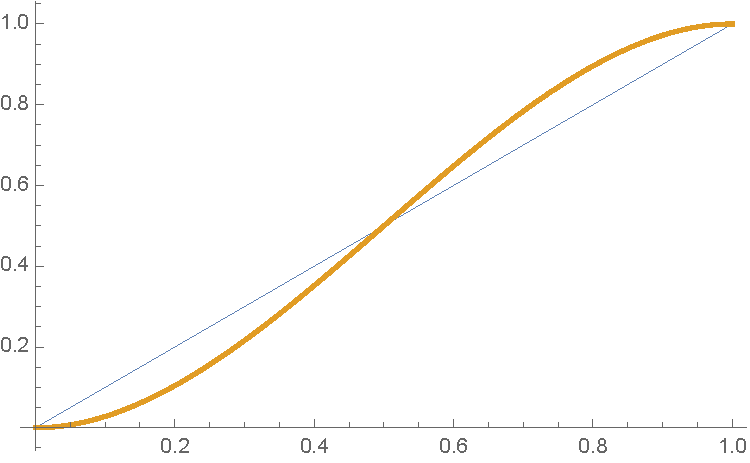
\includegraphics[width=7cm]{fonctionc}
\caption{\label{fig:graph of c}A plot of the function $ x \mapsto \ff(x)$. Notice that it is symmetric with respect to $(1/2,1/2)$ and below the first bisector when $x \in [0,1/2]$.}
\end{center}
\end{figure}

\section{The leaf-growth measure on the Brownian CRT}\label{section:convergence}

In this section we construct the leaf-growth measure $\nu_\mathcal{T}$ on the Brownian CRT and prove that (a scalar multiple of) the latter, equipped with the former, is the scaling limit of the discrete model for the Gromov--Hausdorff--Prokhorov metric. In order to establish the scaling limit, we~provide an explicit description of the spine towards a typical $\nu_\mathcal{T}$-point.

\subsection{Preliminary notation}

The Brownian Continuum Random Tree (CRT) is the random real tree $(\mathcal{T}, d)$ coded by a standard Brownian excursion (length $1$, variance~$1$). This differs by a factor $1/2$ compared to Aldous' original definition. We~refer to \cite{LG2005} for its main properties and for standard notation about real trees, some of which is recalled below. It~is given with a distinguished point $ \rho$ called the \emph{root} of the tree. The degree of a point $x \in \mathcal{T}$ is the number of connected components of $\T\setminus \{x\}$. When the degree is equal to $1$ we say $x$ is a \emph{leaf}; we call $x$ a \emph{point of the skeleton} when its degree is $2$ and a \emph{branch point} when its degree is $3$ (there are almost surely no points with degree $4$ or more in the Brownian CRT). For $x\in \T$, we~call \emph{height} of $x$ its distance to~$\rho$ and denote it by $\h(x)$. We~say that $x$ is a \emph{descendant} of another point $y\in\T$ (and equivalently that $y$ is an \emph{ancestor} of $x$) if $y$ lies on the segment between $\rho$ and $x$, and we call $\T_x$ the subset of $\T$ formed by $x$ and all its descendants. Finally, for $x \in \T$ and $t\geq 0$ we define for the point $[x]_t$ as:
\begin{itemize}
\item the unique ancestor of $x$ with height $t$, if $t< \h(x)$
\item $x$ itself, if $t\geq \h(x)$.
\end{itemize}
In particular, $ \T_{[x]_t}$ denotes the subtree above height $t$ which contains the point $x$. When $[x]_t$ is a branch point and if $t < \h(x)$, then $\T_{[x]_t} \setminus \{[x]_t\}$ has two components and we denote by $ \mathcal{T}_{[x]_{t+}}$ the closure of component that contains~$x$.

The Brownian CRT is also endowed with its uniform mass measure $\mu$ (also called the leaf measure), which can either be seen as the projection of the Lebesgue measure on $[0,1]$ in the coding by the Brownian excursion, or more intrinsically as its natural Hausdorff measure, see \cite{duquesne2005probabilistic,duquesne2006hausdorff}.

In our work, another description of $\mathcal{T}$ will be of key importance. Namely, the Brownian CRT can (with this normalisation) be seen as a fragmentation tree in the sense of Haas and Miermont \cite{HM04} with self-similarity index $\alpha = - \sfrac{1}{2}$ for the dislocation measure
\begin{equation}
\label{eq:Dislocation}
\mathsf{Dis} := \sqrt{\frac{2}{\pi}} \int_{1/2}^{1} \frac{ \mathrm{d}x}{(x(1-x))^{3/2}}\, \delta_{(x,(1-x))}.
\end{equation}
Heuristically, this means that it encodes the genealogy of a system of particles starting from a single particle of mass $1$, where particles of mass $m$ evolve independently and split into two particles of mass $mx$ and $m(1-x)$ at rate $m^{-1/2} \cdot \sqrt{\sfrac{2}{\pi}}\, \pp(x)$, where $\pp(x)$ is as in \eqref{Stirlinglimit}. Following Bertoin \cite{bertoin2002self}, those particles alive at time $t$ correspond to the subtrees of $\T$ above height $t$ and their masses correspond to the $\mu$-masses of those subtrees.

\subsection{Definition of $\nu$}
Conditionally on the CRT~$\mathcal{T}$, the leaf-growth measure $\nu_{\mathcal{T}}$, which throughout this section we will also denote by $\nu$, rendering the dependence on~$\mathcal{T}$ implicit, will be defined by specifying the value $\nu(\T_x)$ for all non-leaf $x\in\T$. Proposition 1 of \cite{Steph13} will then guarantee its existence and uniqueness. The definition will be analogous to the discrete case: there, the relative masses given to the subtrees in an $(a,b)$ split were $C(a,b)$ and $C(b,a)$, and here the relative masses given to the subtrees in a $(x,1-x)$ split will be $\ff(x)$ and $1-\ff(x)=\ff(1-x)$.

Note that the construction is purely deterministic: for the purposes of Proposition~\ref{prop:def:nu}, one can take $\T$ to be any binary compact rooted real tree equipped with a measure $\mu$ supported by the leaves, and $ \mathsf{c}$ to be any symmetric function satisfying $ \mathsf{c}(x) \leq x$ for $x \in [0,1/2]$. Since our only application concerns the Brownian CRT with the specific function $\mathsf{c}=x^2(3-2x)$, for the sake of simplicity we shall keep using the the notations $\mathcal{T}$, $\mu$ and $\ff$ throughout this section, though they should be interpreted here with this more general framework in mind.

Given $x \in \T$, recall from above that we denote by $ \mathcal{T}_{[x]_t}$ and $\mathcal{T}_{[x]_{t+}}$, respectively, the subtree above height $t$ which contains $x$, and in the case of a branch point, the closure of the connected component of $\T\setminus{[x]_t}$ which contains $x$. Finally we set
\[
u_x(t) := \frac{\mu(\T_{[x]_{t+}})}{ \mu(\T_{[x]_t})} \in [0,1].
\]
In particular, since the tree $ \mathcal{T}$ is binary and compact, there are for any \hbox{$x \in \T$}~at~most countably many branch points on the ancestral path of $x$, hence we have \hbox{$u_x(t) < 1$}~only for a countable number of heights $t \leq \h(x)$. In particular, if $(t_i : i \in \mathbb{N})$ is an enumeration of the heights of those branch points then the family \hbox{$ (\mu(\mathcal{T}_{[x]_{t_i}})-\mu(\mathcal{T}_{[x]_{t_i +}}): i \in \mathbb{N})$} is summable, and since the measure $\mu$ does not charge the skeleton, its sum is equal to $1- \mu(\mathcal{T}_x)$. We~deduce then that for all $x \in \T$ we have
\begin{equation} \mu\big(\T_x\big) = \prod_{0 \leq t < \h(x)} u_x(t). \label{eq:noloss}\end{equation}


\subsection{Path towards a typical $\nu$-leaf and spine decomposition}
Recalling the definition of the Brownian dislocation measure in \eqref{eq:Dislocation}, we~now build two measures $\pi_\mu$ and $\pi_\nu$ on $(0,\infty)$ defined by
\begin{align*}
\int_{0}^{\infty} \mathrm{d} \pi_\mu(s) \ \phi(s) &:= \sqrt{\frac{2}{\pi}} \int_{1/2}^{1} \bigl(\ff(x) \phi(-\log (x)) + \ff(1-x) \phi(-\log (1-x))\bigr)\pp(x)\dd x \\
&= \sqrt{\frac{2}{\pi}} \int_0^{1} \ff(x) \phi\left(-\log (x)\right) \pp(x)\dd x
\end{align*}
and
\begin{align*} \int_{0}^{\infty} \mathrm{d} \pi_\nu(s) \ \phi(s) &:= \sqrt{\frac{2}{\pi}} \int_{1/2}^{1}\bigl(\ff(x) \phi(-\log (\ff(x))) + \ff(1-x) \phi(-\log (\ff(1-x)))\bigr)\pp(x)\dd x \\
&= \sqrt{\frac{2}{\pi}} \int_0^{1} \ff(x) \phi\left(-\log (\ff(x))\right)\pp(x)\dd x.
\end{align*}
Consider then $\Pi_\mu$ a Poisson point process (P.p.p.) on $ \mathbb{R}_+ \!\times\! \mathbb{R}_+$ with intensity \hbox{$ \mathrm{d} \pi_\mu \!\otimes\! \mathrm{d}t$}. By replacing each atom $(p,t)$ of $\Pi_\mu$ by the atom $(-\log(\ff (\mathrm{e}^{-p})),t)$ we obtain another Poisson point process with intensity $ \mathrm{d}\pi_\nu \otimes \mathrm{d}t$. We~can then define two coupled (non-decreasing) subordinators $\xi_\mu$ and $\xi_\nu$ started from $0$, and with respective Lévy measures~$\pi_\mu$ and $\pi_\nu$, and obtained by summing the atoms of the respective P.p.p., i.e.,
\begin{equation}\label{defxi}
\xi_\mu(t) = \sum_{\begin{subarray}{c}(p,s) \in \Pi_\mu \\ s \leq t\end{subarray}} p \quad \text{and} \quad \xi_\nu(t) = \sum_{\begin{subarray}{c}(p,s) \in \Pi_\nu \\ s \leq t
\end{subarray}} p = \sum_{\begin{subarray}{c}(p,s) \in \Pi_\mu \\ s \leq t\end{subarray}} -\log(\ff (\mathrm{e}^{-p})).\end{equation}
Then we perform the Lamperti transformation with index $1/2$ using $\xi_\mu:$ we let
\begin{equation}\label{eq:timechange}\theta(t)=\inf\biggl\{u\geq 0: \int_0^u \mathrm{e}^{-\frac12 \xi_{\mu}(r)}\mathrm d r > t\biggr\},\end{equation}
and build two processes $X_\mu$ (a so-called positive self-similar Markov process, see \cite{Lamp62}) and $X_\nu$ (which is not Markovian, since the time change uses information from $X_\mu$) defined for $t\geq0$ by
\begin{equation}
(X_{\mu}(t),X_\nu(t)):=(\mathrm{e}^{-\xi_\mu(\theta(t))},\mathrm{e}^{-\xi_\nu(\theta(t))}). \label{eq:lamperti}\end{equation}
Both of those processes are pure jump and non-increasing from $1$ to $0$, and are absorbed at $0$ at time \begin{equation} \label{def:I} I:=\int_{0}^{\infty}\mathrm{e}^{-\frac12 \xi_\mu(t)}\mathrm{d}t\end{equation} which is almost surely finite since $ \xi_\mu$ drifts to $+\infty$ at linear speed.


\subsection{Scaling limits}\label{sec:scalinglimitproof}
The aim of this section is to prove Theorem \ref{thm:ghpanddim}. For the reader's convenience, we~quickly recall the definition of the (pointed) Gromov--Hausdorff--Prokhorov convergence and refer to \cite{MR3035742,khezeli2020metrization} for more details, as well as \cite{AthreayLorWinter} for a presentation of the topology without the metric. A weighted pointed compact metric space $(M,d,\rho,\mu)$ is a compact metric space equipped with a finite Borel measure $\mu$ and a distinguished point $\rho\in M$. We~let $\mathbb{M}$ be the set of all isometry classes of weighted pointed compact metric spaces. To lighten notation, we~shall often identify a compact weighted metric space with its equivalence class. We~equip $\mathbb{M}$ with the classical Gromov--Hausdorff--Prokhorov metric, defined for every $\boldsymbol{M}:=(M,d, \rho,\mu)$ and $\boldsymbol{M}^{\prime}:=(M^{\prime},d^{{\prime}},\rho^\prime,\mu^{\prime})$ in $\mathbb{M}$ by:
\[
d_{\mathrm{GHP}}\big(\boldsymbol{M},\boldsymbol{M}^{\prime}\big):=\inf\limits_{\phi,\phi^{\prime}}\Bigl(\delta_{\text{H}}\big(\phi(M),\phi^{\prime}(M^{\prime})\vee \delta_{\text{P}}\big(\phi_* \mu,\phi^{\prime}_* \mu^{\prime}\big)\vee \delta(\phi(\rho),\phi^\prime(\rho^\prime)\Bigr),
\]
where the infimum is taken over all isometries $\phi$, $\phi^{\prime}$ from $M$, $M^{\prime}$ into a metric space $(Z, \delta)$ and $\delta_{\text{H}}$ (resp.~$\delta_{\text{P}}$) stands for the classical Hausdorff distance (resp.~the Prokhorov distance) in $Z$. The space $(\mathbb{M},d_{\mathrm{GHP}})$ is then a Polish space.

Our starting point is the well-known convergence in distribution from~\cite{Ald93}:
\begin{equation}\label{eq:gh2pointed} \Bigl(\frac{1}{\sqrt{n}}\tau_n,\rho_n,\mu_n \Bigr) \xrightarrow[\textstyle n\to\infty]{\textstyle(d)} (2\sqrt{2}\,\T,\rho,\mu),
\end{equation}
for the pointed Gromov--Hausdorff--Prokhorov metric, where $\mu_n$ is the uniform measure on the vertices of $\tau_n$. By analogy with this notation, we~shall also use the notation $\nu_n$ for the measure $\nu_{\tau_n}$ introduced in Section~\ref{section:building schemes}. We~saw in Section \ref{section:building schemes} and in Proposition~\ref{prop:def:nu} that the measures $\nu_n$ and $\nu$ are obtained as measurable functions of $(\Psfrac{1}{\sqrt{n}}\tau_n,\rho_n,\mu_n)$ and $(2\sqrt{2}\,\T,\rho,\mu)$ respectively. Furthermore, both measures are constructed similarly by modifying the splitting of the reference measures $\mu_n$ and $\mu$ using the functions $C(a,b)$ and $ \mathsf{c}$. In view of \eqref{eq:gh2pointed} and the convergence \eqref{eq:cc}, it~is natural to expect that those functions are almost ``continuous'', letting us adjoin $\nu_n$ and $\nu$ to~\eqref{eq:gh2pointed} using deterministic arguments.

\begin{figure}[htb] \centering
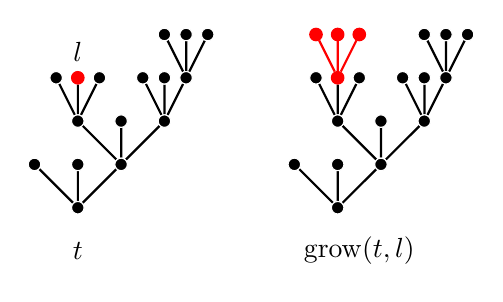
\begin{tikzpicture}[vertex/.style={circle, inner sep=1.6pt, draw=white, fill=black}, gem/.style={diamond, inner sep=1.7pt, fill=green!70!black}, branch/.style={very thick, brown},blossom/.style={green!70!black}, simple/.style={thick}, scale=1.1]
	\begin{pgfonlayer}{nodelayer}
		\node (0) at (5.75,3.25) {$t$};
		\node [style=vertex] (1) at (6.75, 4.75) {};

		\node [style=vertex] (3) at (8.25, 4.25) {};

		\node [style=vertex] (5) at (10, 5.25) {};

		\node [style=vertex] (7) at (6, 5.25) {};
		\node [style=vertex] (8) at (6.25, 4.25) {};
		\node [style=vertex, red, label=above:$l$] (9) at (5.75, 5.25) {};
		\node [style=vertex, red] (11) at (8.5, 5.75) {};
		\node [style=vertex] (12) at (10, 5.75) {};
		\node [style=vertex] (13) at (7, 5.75) {};
		\node [style=vertex] (14) at (7, 5.25) {};
		\node [style=vertex, red] (15) at (8.75, 5.25) {};
		\node [style=vertex] (16) at (9, 5.25) {};
		\node [style=vertex] (17) at (6.75, 5.75) {};
		\node [style=vertex] (21) at (10.25, 5.75) {};
		\node (23) at (9, 3.25) {$\grow(t,l)$};
		\node [style=vertex] (24) at (6.25, 4.75) {};
		\node [style=vertex] (25) at (6.75, 5.25) {};
		\node [style=vertex] (26) at (9.75, 4.75) {};

		\node [style=vertex] (28) at (6.5, 5.25) {};
		\node [style=vertex] (29) at (8.75, 4.75) {};
		\node [style=vertex] (30) at (5.75, 4.75) {};
		\node [style=vertex] (31) at (8.5, 5.25) {};

		\node [style=vertex] (33) at (5.75, 4.25) {};
		\node [style=vertex] (34) at (5.75, 3.75) {};
		\node [style=vertex, red] (35) at (8.75, 5.75) {};
		\node [style=vertex, red] (36) at (9, 5.75) {};
		\node [style=vertex] (37) at (9.25, 4.25) {};
		\node [style=vertex] (38) at (8.75, 4.25) {};
		\node [style=vertex] (39) at (9.75, 5.25) {};
		\node [style=vertex] (40) at (7.25, 5.75) {};
		\node [style=vertex] (41) at (9.25, 4.75) {};
		\node [style=vertex] (42) at (5.25, 4.25) {};
		\node [style=vertex] (43) at (9.5, 5.25) {};
		\node [style=vertex] (44) at (5.5, 5.25) {};
		\node [style=vertex] (45) at (9.75, 5.75) {};
		\node [style=vertex] (46) at (8.75, 3.75) {};

	\end{pgfonlayer}
	\begin{pgfonlayer}{edgelayer}
		\draw [style=simple] (29) to (37);
		\draw [style=simple] (43) to (26);
		\draw [style=simple] (45) to (5);
		\draw [style=simple] (31) to (29);
		\draw [style=simple] (44) to (30);
		\draw [style=simple, red] (11) to (15);
		\draw [style=simple] (13) to (14);
		\draw [style=simple] (41) to (37);
		\draw [style=simple] (8) to (34);
		\draw [style=simple] (30) to (8);
		\draw [style=simple] (5) to (26);
		\draw [style=simple, red] (35) to (15);
		\draw [style=simple] (38) to (46);
		\draw [style=simple] (28) to (1);
		\draw [style=simple] (1) to (8);
		\draw [style=simple] (25) to (1);
		\draw [style=simple] (16) to (29);
		\draw [style=simple] (24) to (8);
		\draw [style=simple] (3) to (46);
		\draw [style=simple] (15) to (29);
		\draw [style=simple] (17) to (14);
		\draw [style=simple] (21) to (5);

		\draw [style=simple] (12) to (5);

		\draw [style=simple] (40) to (14);
		\draw [style=simple] (37) to (46);
		\draw [style=simple] (7) to (30);

		\draw [style=simple] (42) to (34);
		\draw [style=simple] (26) to (37);

		\draw [style=simple] (9) to (30);

		\draw [style=simple] (14) to (1);
		\draw [style=simple] (33) to (34);
		\draw [style=simple] (39) to (26);
		\draw [style=simple, red] (36) to (15);
	\end{pgfonlayer}
\end{tikzpicture}
\caption{\label{fig:leaf growth}A plane ternary tree of size 5 (i.e., with 5 internal vertices and thus $3+2\cdot 4 =11$ leaves) is grown at the leaf $l$ by adding 3 children to $l$, thus creating the tree $\grow(t,l)$ of size 6.}
\end{figure}

\section{Building schemes for trees: leaf-growth measures}\label{section:building schemes}

In this section, we~set up some notation and give some context for what we are about to discuss, i.e., how to ``uniformly grow'' trees ``from their leaves''. For completeness, we~shall state some known results in their general form, which involves $d$-ary trees (see~Luczak \& Winkler \cite{LW04}).

In the case $d=2$, motivated by applications to the study of mixing times of flip chains, this procedure has been made completely explicit by Caraceni and Stauffer \cite{CS20} and forms the basis of the current work.

\Subsection{Building schemes for $d$-ary trees}

\begin{defn}\label{def:complete d-ary tree}
Let $d\!\geq\! 2$ and $n\!\geq\! 0$ be integers. We~shall call a \emph{$d$-ary tree of size~$n$} a rooted plane tree whose vertices all have $d$ children (we call such vertices \emph{internal}) or no children (we call such vertices \emph{leaves}).

We say that a $d$-ary tree $\tau$ has \emph{size} $|\tau|=n$ if it has $n$ internal vertices. For simplicity, we~shall commit a slight abuse of notation and also write $\tau$ for the set of vertices of~$\tau$, so we can write $v\in \tau$ to mean that $v$ is a vertex of $\tau$.

We call $\sT_n^{(d)}$ the set of all $d$-ary trees of size $n$ and write $\sT^{(d)}$ for $\bigcup_{n\geq 0}\sT_n^{(d)}$. Note that the set $\sT^{(d)}_0$ contains one element, the tree consisting of only its root.
\end{defn}

A $d$-ary tree has a natural recursive structure: if $t\in\sT_n^{(d)}$ with $n\geq 1$, it~naturally induces a sequence of $d$-ary trees $(t^1,\ldots, t^d)$: letting $\rho\in t$ be the root, one can erase all children of $\rho$ other than the $i$th child $v_i$ and consider the connected component of~$v_i$, rooted at $v_i$, to obtain $t^i$. One then has $\sum_{i=1}^d|t^i|=n-1$. From this decomposition one obtains the \emph{profile} of the tree $t$:

\begin{defn}
Given $t\in \sT_n^{(d)}$ with $n\geq 1$, its \emph{profile} is the vector $\underline{x}(t)=(|t^1|,\ldots,|t^d|)\in \mathbb{N}^d$.	
\end{defn}

Note that the term profile is often used with different meanings (for example, for the sequence of generation sizes) in similar contexts; however, we~choose to employ it here to keep notation at least partially consistent with the original paper \cite{LW04}.

We now discuss a particular ``growth'' operation on $d$-ary trees. Given a pair $(t,l)$, where $t$ is a $d$-ary tree of size $n$ and $l$ is a leaf of $t$, we~construct a tree $\grow(t,l)$ of size $n+1$ by adding $d$ leaves to $t$ as children of the vertex $l$, thus turning $l$ into an internal vertex.

Luczak and Winkler consider the following natural question in \cite{LW04}: supposing~$\tau_n$ is a uniform random element of $\sT^{(d)}_n$ and $\tau_{n+1}$ is a uniform random element of $\sT^{(d)}_{n+1}$, is it possible to couple $\tau_n$ and $\tau_{n+1}$ in such a way that $\tau_{n+1}$ is always of the form $\grow(\tau_n,l_n)$, where $l_n$ is some leaf of the tree $\tau_n$?

They call a family of such couplings for all $n\geq 0$ a \emph{building scheme} for $d$-ary trees and answer the question in the affirmative, thus proving


\begin{thm}\label{thm:ghpanddim} We have the following convergence in distribution for the Gromov--Hausdorff--Prokhorov topology (see Section \ref{sec:scalinglimitproof} for a definition):\vspace*{-3pt}
\[
\bigl(n^{-1/2} \cdot \tau_n, \nu_{\tau_n} \bigr) \xrightarrow[\textstyle n\to \infty]{\textstyle (d)}(2\sqrt{2}\,\mathcal{T}, \nu_{ \mathcal{T}}),
\]
where $ \mathcal{T}$ is the Brownian CRT and $\nu_{\mathcal{T}}$ is a probability measure on the leaves of $\T$ with Hausdorff dimension $2\gamma= 6(2- \sqrt{3}) \approx 1.6077$.
\end{thm}

\begin{prop}[Definition of $\nu$]\label{prop:def:nu} Suppose that $ \mathcal{T}$ is a compact binary rooted tree equipped with a measure $\mu$ supported by its leaves. If $\mathsf{c}:[0,1] \to [0,1]$ is symmetric with respect to $1/2$ and satisfies $ \mathsf{c}(x) \leq x$ for $x \in [0,1/2]$, then there exists a unique Borel measure $\nu$ supported by the leaves of $ \mathcal{T}$ specified by
\begin{equation} \nu(\T_x) := \prod_{0 \leq t < \h(x)} \ff(u_x(t)).
\end{equation}
\end{prop}
\begin{proof} Let, for $x\in\T$, $m(x)=\prod_{0 \leq t < \h(x)} \ff(u_x(t))$. Since we have $ \mathsf{c}(x) \leq x$ for $x \in [0,1/2]$ the product is well-defined and is non-zero as soon as $\prod_{0 \leq t < \h(x)} u_x(t)$ is non-zero. One can straightforwardly check the following:
\begin{itemize}
\item $m$ is a well-defined and nonnegative function, which is equal to $0$ exactly on the leaves of $ \mathcal{T}$.
\item $m$ is non-increasing, in~the sense that, if $x$ is an ancestor of $y$, then $m(x)\geq m(y)$.
\item $m$ is ``left-continuous'', in~the sense that $m(x)=\lim_{s\to (\mathrm{ht}(x))^{-}} m([x]_s)$.
\item $m$ is ``additively right-continuous'': if $x$ is not a branch point, then $m$ is continuous at $x$, while if $x$ is a branch point, then, letting $y$ and $z$ be two descendants of $x$ not in the same one of the two subtrees originating at $x$, then $m(x)= \lim_{s\to (\mathrm{ht}(x))^+} m([y]_s)+\nobreak m([z]_s)$.
\end{itemize}
These facts, combined, let us use \cite[Prop.\,1]{Steph13}, which then tells us there exists a unique measure $\nu$ such that $\nu(\T_a)=m(a)$ for $a$, and that it has no atoms. With the notation introduced just before the Proposition, since $\mu$ does not charge the skeleton, we~can also check that $1-\nu(\mathcal{T}_x) = \sum_{i \in \mathbb{N}} \big(\nu (\mathcal{T}_{[x]_{t_i}}) -\nu (\mathcal{T}_{[x]_{t_i +}})\big)$, in~particular $\nu$ gives no mass to the ancestral path of $x$, and as a result is supported by the leaves of $ \mathcal{T}$.
\end{proof}

\begin{thm}[Spine decomposition]\label{thm:spinedec} Conditionally on the Brownian CRT $ \mathcal{T}$, let~$L$ be a $\nu$-distributed random point of $\tbr$. Then the bivariate process
\[
(\mu(\T_{[L]_{t+}}),\nu(\T_{[L]_{t+}}))_{t\geq 0}
\]
(under the annealed law) is distributed as $(X_{\mu},X_{\nu})$.
As a consequence, $L$ is almost surely a leaf, and its height has the law of $I$.

Moreover, let $(t_i,i\in\N)$ be the times at which $u_L(\cdot) \in (0,1)$, and for all $i\in \N$ let~$\T_i$ be the subtrees which branch off $\llbracket \rho,L\rrbracket$ at those times (ranked, say in decreasing order of their $\mu$-masses). Then, conditionally on the whole process $(\mu(\T_{[L]_{t}}),t\geq 0)$, the trees
\[
\big(u_L(t_i) \cdot \mu(\T_{L(t_i)}) \big)^{-1/2} \cdot \T_i, \quad i \geq 1,
\]
are independent Brownian CRT's.
\end{thm}

\begin{proof}
Informally, the idea is that the path to $L$ encounters binary splits at the same rate as the path to a uniform leaf, but crosses those splits differently, using the probability $\ff$. This is formalised in \cite{PitmanWinkel2013} by the notion of \emph{bifurcator}. If $L'$ is a leaf with distribution $\mu$, then the paths from $\rho$ to $L$ and to $L'$ will encounter countable numbers of binary branch points. At any common such branch point, let $x$ and $1-x$ be the relative $\mu$-masses of both pending subtrees, choosing $x$ to be the mass of the one containing $L$. Then the probability that $L'$ is in the other subtree, known as the ``switching probability'' in \cite{PitmanWinkel2013}, is equal to $\ff(1-x)$. While the process $(Y(t),t\geq 0)$ defined by $Y(t)=\mu(\T_{[L']_{t+}})$ is well-known \cite[\S 4]{bertoin2002self} to be the Lamperti transform of a subordinator with Lévy measure $\pi_{\mathrm{unif}}$, defined by
\begin{align*}
\int_{0}^{\infty} \mathrm{d} \pi_{\mathrm{unif}}(s) \ \phi(s) &= \sqrt{\frac{2}{\pi}} \int_{1/2}^{1} \bigl(x \phi(-\log (x)) + (1-x) \phi(-\log (1-x))\bigr)\pp(x)\dd x \\
&= \sqrt{\frac{2}{\pi}} \int_0^{1} x \phi(-\log (x))\pp(x)\dd x,
\end{align*}
Proposition 1 from \cite{PitmanWinkel2013} states then that the process $\mu(\T_{[L]_{t+}}),t\geq 0$ will be the Lamperti transform of a subordinator where the initial $x$ in the integrand of the above is replaced by $\ff(x)$, giving us $\pi_\mu$.

That $(\nu(\T_{[L]_{t+}}),t\geq 0)$ has the appropriate paired distribution comes from the fact that its multiplicative jumps are obtained by applying $\ff$ to those of $(\mu(\T_{[L]_{t+}}),t\geq 0)$, which is how $X_{\nu}$ is derived from $X_{\mu}$.

Finally, the spinal decomposition itself is again a consequence of \cite{PitmanWinkel2013}, this time Lemma 21.
\end{proof}

\begin{prop}\label{prop:continuous Hausdorff} Almost surely for $\mathcal{T}$ and a.e.\ for $\nu(\mathrm{d}\ell)$ we have
\[
\lim_{r \to 0} \frac{\log \nu \big(B_r(\ell)\big) }{\log r} = 2 \dH.
\]
\end{prop}

\begin{proof}
Recall that $\gamma=3(2-\sqrt{3})$, and the definitions of $\pp(x)$ in \eqref{Stirlinglimit}, $\cc(x)$ in~\eqref{eq:cc}, $\xi_\mu$~and~$\xi_\nu$ in \eqref{defxi}, $X_\mu$ and $X_\nu$ in \eqref{eq:lamperti}, the time change $\theta$ in~\eqref{eq:timechange} and extinction time $I$ in~\eqref{def:I}. By Theorem \ref{thm:spinedec}, we~can assume that the bivariate process $(\mu(\T_{[L]_{t+}}),\nu(\T_{[L]_{t+}}))_{t\geq 0}$ is given by $(X_\mu,X_\nu)$.

The local rate of growth of $\nu$ near a $\nu$-typical point is related to the asymptotic behaviour of $X_\mu$ and $X_\nu$ near their extinction time. To understand this, let us compute the first moments of the Lévy processes $\xi_\mu$ and $\xi_\nu:$ we have
\[
\mathbb{E}[\xi_\mu(t)] = t \int_0^{\infty} s\ \mathrm{d}\pi_\mu(s) = \sqrt{2 \pi} \quad \text{and}\quad \mathbb{E}[\xi_\nu(t)] = t \int_0^{\infty} s\ \mathrm{d}\pi_\nu(s) = \dH \sqrt{2\pi}.
\]
Since the Lévy measure integrates the identity function, by the law of large numbers we have $t^{-1}\xi_\mu (t) \to \sqrt{2 \pi}$ and $t^{-1}\xi_\nu (t) \to \dH \sqrt{2\pi}$ as $t \to \infty$ almost surely. Through the Lamperti transformation \eqref{eq:lamperti}, this turns into estimate on the time change $\theta$ since for $\veps>0$,
\[
\int_{\theta(I-\veps)}^{\infty} \mathrm{e}^{-\frac12 \xi_\mu(t)}\mathrm dt=\veps,
\]
from which we straightforwardly deduce using the above law of large numbers that
\[
\theta(I-\veps)\underset{\veps\to 0}\sim-\frac2{\sqrt{2\pi}}\log \veps
\]
almost surely. Substituting back into \eqref{eq:lamperti}, we~find using the same law of large numbers that
\[
\lim_{ \varepsilon \to 0}\frac{\log X_\mu(I - \varepsilon)}{\log \varepsilon} =2\quad \text{and} \quad \lim_{ \varepsilon \to 0}\frac{\log X_\nu(I - \varepsilon)}{\log \varepsilon} = 2\dH,
\]
also almost surely.

Now, by the first item of the spine decomposition (Theorem \ref{thm:spinedec}), we~clearly have $\nu\big(B_{ \varepsilon }(L)\big) \leq X_\nu(I - \varepsilon)$ as a process in $ \varepsilon$ and together with the last display this entails that
\[
\liminf_{ \varepsilon \to 0} \frac{\log \nu \big(B_\varepsilon(L)\big) }{\log \varepsilon} \geq 2 \dH, \quad \text{a.s.}.
\]
Let us now prove the upper bound for the dimension via a lower bound on $\nu \big(B_\varepsilon(L)\big)$. For this, we~concentrate on jumps of $\xi_\mu$ of size at least $\log 2$. Remember that thanks to the spine decomposition, conditionally on such a jump of size $s\geq \log 2$ appearing at time $t$, the subtree $\T_{[L]_{u}}\setminus \T_{[L]_{u+}} \cup \{[L]_{u}\}$ with $t=\theta(u)$ (which is the subtree which is ``left on the side'' at height $u$) is an independent Brownian CRT with $\mu$-mass
\[
(1- \mathrm{e}^{-s}) \mathrm{e}^{- \xi_\mu(t-)} \geq \frac{1}{2}\, \mathrm{e}^{- \xi_\mu(t-)}.
\]
Notice two things: first, the $\nu$-mass of this subtree is at least $ \mathrm{e}^{- \xi_\nu(t-)}/2$ (because $\ff(x) \leq x$ for $x \in [0,1/2]$) and second, this tree has a fixed probability equal to $ \mathbb{P}(\h(\mathcal{T}) \leq 1)$ of being of height less than the square root of its $\mu$-mass. Under those conditions, this subtree is a subset of $B_{ \varepsilon}(L)$ for $\varepsilon \geq \mathrm{e}^{-\frac12 \xi_\mu(t-)} + \int_{t}^\infty \mathrm{e}^{-\frac12 \xi_\mu(s)} \mathrm{d}s$ and we have
\begin{equation} \label{eq:lowerbound12}\nu \big(B_{ \varepsilon}(L)\big) \geq \frac12\, \mathrm{e}^{- \xi_\nu(t-)}.
\end{equation} By the law of large numbers on $\xi_\mu$ and $\xi_\nu$, we~can take $\varepsilon = c_1 \mathrm{e}^{- t \sqrt{2\pi}/2}$ and we have $\nu \big(B_{ \varepsilon}(L)\big) \geq c_2 \mathrm{e}^{- t \sqrt{2\pi} \gamma/2} = \varepsilon^{2\gamma + o(1)}$ for some $c_1,c_2>0$. The preceding inequality is only valid for those $ \varepsilon$ associated to a jump time $t$ satisfying the above conditions. However, if we can find a family $t_i \to \infty$ of such times satisfying
\begin{equation} \label{eq:goaldensity} 0 < t_1 < t_2 < \cdots < t_i \xrightarrow[\textstyle i \to \infty]{} \infty \quad \text{and} \quad\lim_{t \to \infty} \frac{t_{i+1}}{t_i} =1,
\end{equation}
then the bound $\nu \big(B_{ \varepsilon}(L)\big) \geq \varepsilon^{2\gamma + o(1)}$ still holds as $ \varepsilon \to 0$ and proves the lower bound on the Hausdorff dimension. To see \eqref{eq:goaldensity}, notice that in the time parametrisation of~$\xi_\nu$, the intensity $C>0$ of such times is positive: by a standard law of large numbers we can almost surely find a diverging sequence of jump times $t_i$ satisfying all of the above assumptions and which satisfy $t_i \sim C i$. This entails \eqref{eq:goaldensity} and completes the proof.
\end{proof}

\begin{proof}[Proof of Theorem \ref{thm:ghpanddim}]
Using the Skorokhod representation theorem, we~can assume that \eqref{eq:gh2pointed} holds almost surely, and the proof will proceed deterministically. Next, by a general representation theorem for Gromov-Hausdorff-type topologies~\cite[Lem.\,2.5]{khezeli2023unified}, we~can
embed all trees $\tau_n$ and $ \mathcal{T}$ isometrically in the same compact
metric space $(E,d_E)$---we keep the same notation for simplicity---, in~such a way that
\begin{equation*}
\Bigl(\frac{1}{\sqrt{n}} \tau_n,\rho_n,\mu_n\Bigr) \xrightarrow[\textstyle n\to\infty]{} (2\sqrt{2}\,\T,\rho,\mu),
\end{equation*}
holds in pointed Hausdorff-Prokhorov sense inside $E$. Fix then any point $x$ in the skeleton of $\T$ which is not a branch point. Lemma \ref{lemma:annoyingmetricthing} shows that there exists a sequence $(x_n,n\in\N)$ with $x_n\in\tau_n$ such that $x_n \to x$ in $E$ and $\mu_n((\tau_n)_{x_n}) \to \mu(\T_x)$. We~will now show that we also have
\begin{equation}\label{eq:GHPlimofnu} \lim_{n \to \infty} \nu_n((\tau_n)_{x_n})= \nu(\T_x),\end{equation}
which will guarantee via the Portmanteau theorem and \cite[Prop.\,1]{Steph13}, that any subsequential limit of $(\nu_n)$ is equal to $\nu$, ending the proof of Theorem \ref{thm:ghpanddim} since $ \mathcal{T}$ is compact.

Let us denote by $h_n$ the height of $x_n$ and by $(a^{(n)}_i,b^{(n)}_i)$ the sizes of the two subtrees above the ancestor of $x_n$ at height $0\leq i < h_n$, with the convention that $a^{(n)}_i$ is the size of the subtree containing $x_n$. It~is then straightforward, but rather long, to prove that we also have the convergence\vspace*{-3pt}\enlargethispage{\baselineskip}
\begin{equation} \label{eq:pointlimit} \biggl(\Bigl(\frac{a_i^{(n)}}{a_i^{(n)}+b_i^{(n)}} , \frac{i}{ 2\sqrt{2n}} \Bigr) : 0 \!\leq\! i \!<\! h_n \biggr) \xrightarrow[\textstyle n \to \infty]{}\biggl(\Bigl(\frac{\mu(\T_{[x]_{t+}})}{\mu(\T_{[x]_{t}})},t \Bigr) : 0 \!\leq\! t\! <\! \mathrm{ht}(x) \biggr)
\end{equation}
in terms of point processes on $ \mathbb{R}_+^* \times \mathbb{R}_+$. In particular, recall that \eqref{eq:noloss} holds almost surely.
Recall first from the construction of $\nu_n$ and $\mu_n$ that we have\vspace*{-3pt}
\begin{equation} \label{rappelnun} \nu_n((\tau_n)_{x_n}) = \prod_{i=0}^{h_n-1} C(a_i^{(n)}, b_i^{(n)}) \quad \text{and} \quad \mu_n((\tau_n)_{x_n}) = \prod_{i=0}^{h_n-1} \frac{a_i^{(n)}}{a_i^{(n)}+b_i^{(n)}+1}.
\end{equation}
On the continuous side, if we set $a_t = \mu(\T_{[x]_{t+}})$ and $b_t = \mu(\T_{[x]_{t}})-\mu(\T_{[x]_{t+}})$ for $0 \leq t \leq \mathrm{ht}(x)$ (note that $b_t=0$ when $[x]_t$ is not a branch point), then by \eqref{eq:noloss} and Proposition \ref{prop:def:nu} we have\vspace*{-3pt}
\begin{equation} \label{rappelnu}\nu(x) = \prod_{t < \mathrm{ht}(x)} \mathsf{c}(\spfrac{a_t}{a_t+b_t}) \quad \text{and} \quad \mu(x) = \prod_{t < \mathrm{ht}(x)} \frac{a_t}{a_t+b_t}.
\end{equation}
On the one hand, the convergences \eqref{eq:pointlimit}, \eqref{eq:cc} and Fatou's lemma directly imply that\vspace*{-3pt}
\[
\limsup_{n \to \infty} \nu_n((\tau_n)_{x_n}) = \limsup_{n \to \infty}\prod_{i=0}^{h_n-1} C(a_i^{(n)}, b_i^{(n)}) \leq \prod_{t < \mathrm{ht}(x)} \mathsf{c}(\spfrac{a_t}{a_t+b_t}) =\nu(x).
\]
To get the matching lower bound $\nu(x)\leq \liminf_{n \to \infty} \nu_n((\tau_n)_{x_n})$, notice that the same argument yields\vspace*{-3pt}
\[
\limsup_{n \to \infty} \mu_n((\tau_n)_{x_n}) = \prod_{i=0}^{h_n-1} \frac{a_i^{(n)}}{a_i^{(n)}+b_i^{(n)}+1} \leq \mu(x) = \prod_{t < \mathrm{ht}(x)} \frac{a_t}{a_t+b_t};
\]
here, however, we~know that the matching lower bound holds since\vspace*{-3pt}
\[
\lim_{n \to \infty} \mu_n((\tau_n)_{x_n}) = \mu(\mathcal{T}_x)
\]
is known. Using the fact that $C(a,b) \geq \spfrac{a}{a+b+1}$ for $a \geq b$, we~deduce that\vspace*{-3pt}
\[
1\geq \lim_{\varepsilon \to 0} \prod_{i=0}^{h_n-1} C(a_i^{(n)}, b_i^{(n)})\mathbf{1}_{b_i^{(n)} \leq \varepsilon a_i^{(n)}} \geq \lim_{\varepsilon \to 0} \prod_{i=0}^{h_n-1} \frac{a_i^{(n)}}{a_i^{(n)}+b_i^{(n)}+1}\mathbf{1}_{b_i^{(n)} \leq \varepsilon a_i^{(n)}} = 1,
\]
from which \eqref{eq:GHPlimofnu} follows.
\end{proof}

\section{Limits of trees and subtrees}

\begin{lem}\label{lemma:annoyingmetricthing}
Consider a sequence $((\T_n,\rho_n,\mu_n),n\in\N)$ of deterministic rooted $\R$\nobreakdash-trees which are subsets of a fixed compact metric space $(E,d)$, such that $\T_n\to \T$, $\rho_n\to \rho$ and $\mu_n\to\mu$ for respectively the Hausdorff metric $d_{\mathrm{H}}$ on compact subsets of~$E$, the metric $d$ on $E$, and the Prokhorov metric $d_{\mathrm{P}}$ for Borel probability measures on $E$.
Then, for any $z\in\T$, there exists a sequence $(z_n,n\in\N)$ with $z_n\in T_n$ such that $z_n\to z$ and $\mu_n((\T_n)_{z_n}) \to \mu(\T_z)$.
\end{lem}

\begin{proof}
Write
\[
\veps_n := 2 \max\bigl(d_{\mathrm{H}}(\T_n,\T) , d(\rho_n,\rho), d_{\mathrm{P}}(\mu_n,\mu)\bigr),
\]
this tends to $0$ as $n$ tends to infinity.

Let $h$ be the height of $z$, for all $n$, $x_n$ an element of $\T_n$ such that $d(z_n,x_n)\leq \veps_n$, and $y_n$ be the ancestor of $x_n$ in $\T$ with height $\mathrm{ht}(x_n)-\veps_n$, Notice that $d(y_n,z)\leq 3\veps_n$

Let us show that $(\T_n)_{y_n}$ converges to $T_z$ for the Hausdorff metric. We~use the notation $A^{\veps}$ to denote the $\veps$-enlargement of a subset $A$ of $E$ and will show that we have both $\T_z\subset (\T_n)_{y_n}^{\veps_n}$ and $(\T_n)_{y_n}\subset \T_z^{\veps'_n}$ with $\veps'_n\to 0$.

Let $a\in \T_z$, we~know that there is $b\in \T_n$ such that $d(a,b)\leq \veps_n$, and we will show that $b$ is in $(\T_n)_{y_n}$. By the triangle inequality we have $d(b,x_n)\leq d(b,a)+d(a,z)+d(z,x_n)\leq d(a,z)+2\veps_n$ and $d(a,z)\leq d(b,x_n)+2\veps_n$, hence $|d(b,x_n)-d(a,z)|\leq x\veps'_n$. Similarly we obtain $|d(b,\rho_n)-d(a,\rho)|\leq 2\veps_n$ and $|d(x_n,\rho_n)-d(z,\rho)|\leq 3\veps_n$ Since $d(a,\rho)+d(a,z)+d(z,\rho)$, we~deduce that $d(b,x_n)+d(x_n,\rho_n)-d(b,\rho_n)\leq 6\veps_n$. Since~$\T_n$ is an $\R$-tree, we~can see that this difference is equal to twice the the distance from~$x_n$ to its most recent common ancestor with $b$ is at most $3\veps_n$, hence this most recent common ancestor is a descendant of $y_n$, hence $b\in (\T_n)_{y_n}$, hence $\T_z\subset (\T_n)_{y_n}^{\veps_n}$.

Similarly, omitting the details, it~can be seen that $(\T_n)_{y_n}\subset \T_{u_n}$, where $u_n$ is an ancestor of $z$ such that $d(u_n,z)\to 0$. However, since $\T$ is compact, we~deduce that $\T_{u_n}\subset \T_z^{\veps'_n}$, where $\veps'_n$ tends to $0$, otherwise there would be a sequence with no subsequential limits.

We can now finish the proof. Letting $\eta_n=\max(\veps_n,d_{\mathrm{H}}((\T_n)_{y_n},T_z))$ for all $n$, we~have $\T_z\subset (\T_n)^{\veps_n}_{z'_n}$, we~now finally define $z_n$ as the ancestor of $z'_n$ such that $\mathrm{ht}(z_n)=\mathrm{ht}(z'_n)-\eta_n$. The same argument as in the previous paragraph shows that $(\T_n)_{z_n}$ converges to $\T_z$ for the Hausdorff distance, hence $\eta'_n:=\max(\eta_n,d_{\mathrm{H}}((\T_n)_{z_n},T_z))$ tends to $0$, and we have the following inclusions of sets:
\[
\T_z\subset (\T_n)_{z'_n}^{\eta_n} \subset (\T_n)_{z_n} \subset \T_z^{\eta'_n}.
\]
By the definition of the Prokhorov metric on measures, we~then have
\[
\mu(\T_z)\leq \mu_n((\T_n)_{z_n})+\eta_n\leq \mu(\T_z^{\eta'_n})+\eta_n+\eta'_n.
\]
However, since $\T_z$ is a closed set, $\mu(\T_z^{\eta'_n})$ converges to $\mu(\T_z)$, and by the sandwich theorem, so does $\mu_n((\T_n)_{z_n})$.
\end{proof}

\begin{thebibliography}{99}
\bibitem{addario2014growing} L. Addario-Berry - “Growing random 3-connected maps” , Electron. Comm. Probab. 19 (2014), article ID 54, 12 pages
\bibitem{MR3035742} R. Abraham, J.-F. Delmas \& P. Hoscheit - “A note on the Gromov-Hausdorff-Prokhorov distance between (locally) compact metric measure spaces” , Electron. J. Probab. 18 (2013), article ID 14, 21 pages
\bibitem{Ald91a} D. Aldous - “The continuum random tree. I” , Ann. Probab. 19 (1991) no. 1, p. 1-28
\bibitem{Ald91} D. Aldous - “The continuum random tree. II. An overview” , in Stochastic analysis (Durham, 1990) , London Math. Soc. Lecture Note Ser. , vol. 167 , Cambridge Univ. Press, Cambridge, 1991, p. 23-70
\bibitem{Ald93} D. Aldous - “The continuum random tree. III” , Ann. Probab. 21 (1993) no. 1, p. 248-289
\bibitem{AthreayLorWinter} S. Athreya, W. Löhr \& A. Winter - “The gap between Gromov-vague and Gromov–Hausdorff-vague topology” , Stochastic Process. Appl. 126 (2016) no. 9, p. 2527-2553
\bibitem{bacher2017efficient} A. Bacher, O. Bodini \& A. Jacquot - “Efficient random sampling of binary and unary-binary trees via holonomic equations” , Theoret. Comput. Sci. 695 (2017), p. 42-53
\bibitem{bertoin2002self} J. Bertoin - “Self-similar fragmentations” , Ann. Inst. H. Poincaré Probab. Statist. 38 (2002) no. 3, p. 319-340
\bibitem{billingsley1965} P. Billingsley - Ergodic theory and information , Wiley Series in Probab. and Math. Stat. , Wiley, 1965
\bibitem{BK14} J. Bertoin \& I. Kortchemski - “Self-similar scaling limits of Markov chains on the positive integers” , Ann. Appl. Probab. 26 (2016) no. 4, p. 2556-2595
\bibitem{CFT25} N. Curien, W. Fleurat \& A. Twigt - “Growing self-similar Markov trees” , 2025, work in progress
\bibitem{CurienHaas} N. Curien \& B. Haas - “The stable trees are nested” , Probab. Theory Relat. Fields 157 (2013) no. 3-4, p. 847-883
\bibitem{CLGharmonic} N. Curien \& J.-F. Le Gall - “The harmonic measure of balls in random trees” , Ann. Probab. 45 (2017) no. 1, p. 147-209
\bibitem{Carmona/Petit/Yor} P. Carmona, F. Petit \& M. Yor - “On the distribution and asymptotic results for exponential functionals of Lévy processes” , in Exponential functionals and principal values related to Brownian motion , Bibl. Rev. Mat. Iberoamericana , Revista Matemática Iberoamericana, Madrid, 1997, p. 73-130
\bibitem{CS20} A. Caraceni \& A. Stauffer - “Polynomial mixing time of edge flips on quadrangulations” , Probab. Theory Relat. Fields 176 (2020) no. 1-2, p. 35-76
\bibitem{CS23} A. Caraceni \& A. Stauffer - “Growing uniform planar maps face by face” , Random Structures Algorithms 63 (2023) no. 4, p. 942-967
\bibitem{duquesne2005probabilistic} T. Duquesne \& J.-F. Le Gall - “Probabilistic and fractal aspects of Lévy trees” , Probab. Theory Relat. Fields 131 (2005) no. 4, p. 553-603
\bibitem{duquesne2006hausdorff} T. Duquesne \& J.-F. Le Gall - “The Hausdorff measure of stable trees” , Alea 1 (2006), p. 393-415
\bibitem{MR2221786} S. N. Evans, J. Pitman \& A. Winter - “Rayleigh processes, real trees, and root growth with re-grafting” , Probab. Theory Relat. Fields 134 (2006) no. 1, p. 81-126
\bibitem{EW06} S. N. Evans \& A. Winter - “Subtree prune and regraft: a reversible tree-valued Markov process” , Ann. Probab. 34 (2006) no. 3, p. 81-126
\bibitem{FPRW18} N. Forman, S. Pal, D. Rizzolo \& M. Winkel - “Aldous diffusion I: a projective system of continuum $k$ -tree evolutions” , 2018
\bibitem{FPRW20} N. Forman, S. Pal, D. Rizzolo \& M. Winkel - “Projections of the Aldous chain on binary trees: intertwining and consistency” , Random Structures Algorithms 57 (2020) no. 3, p. 745-769
\bibitem{forman2023aldous} N. Forman, S. Pal, D. Rizzolo \& M. Winkel - “The Aldous diffusion: a stationary evolution of the Brownian CRT” , 2023
\bibitem{goldschmidt2019parking} C. Goldschmidt \& M. Przykucki - “Parking on a random tree” , Combin. Probab. Comput. 28 (2019) no. 1, p. 23-45
\bibitem{HM04} B. Haas \& G. Miermont - “The genealogy of self-similar fragmentations with negative index as a continuum random tree” , Electron. J. Probab. 9(4) (2004), p. 57-97
\bibitem{HM12} B. Haas \& G. Miermont - “Scaling limits of Markov branching trees with applications to Galton-Watson and random unordered trees” , Ann. Probab. 40 (2012) no. 6, p. 2589-2666
\bibitem{HS14} B. Haas \& R. Stephenson - “Scaling limits of $k$ -ary growing trees” , Ann. Inst. H. Poincaré Probab. Statist. 51 (2015) no. 4, p. 1314-1341
\bibitem{khezeli2020metrization} A. Khezeli - “Metrization of the Gromov–Hausdorff(-Prokhorov) topology for boundedly-compact metric spaces” , Stochastic Process. Appl. 130 (2020) no. 6, p. 3842-3864
\bibitem{khezeli2023unified} A. Khezeli - “A unified framework for generalizing the Gromov-Hausdorff metric” , Probab. Surv. 20 (2023), p. 837-896
\bibitem{Lamp62} J. Lamperti - “Semi-stable stochastic processes” , Trans. Amer. Math. Soc. 104 (1962), p. 62-78
\bibitem{lawler1993discrete} G. F. Lawler - “A discrete analogue of a theorem of Makarov” , Combin. Probab. Comput. 2 (1993) no. 2, p. 181-199
\bibitem{LG2005} J.-F. Le Gall - “Random trees and applications” , Probab. Surv. 2 (2005), p. 245-311
\bibitem{lohr2020aldous} W. Löhr, L. Mytnik \& A. Winter - “The Aldous chain on cladograms in the diffusion limit” , Ann. Probab. 48 (2020) no. 5, p. 2565-2590
\bibitem{lyons1995ergodic} R. Lyons, R. Pemantle \& Y. Peres - “Ergodic theory on Galton–Watson trees: speed of random walk and dimension of harmonic measure” , Ergodic Theory Dynam. Systems 15 (1995) no. 3, p. 593-619
\bibitem{lyons2008growth} R. Lyons, R. Peled \& O. Schramm - “Growth of the number of spanning trees of the Erdős–Rényi giant component” , Combin. Probab. Comput. 17 (2008) no. 5, p. 711-726
\bibitem{LW04} M. Luczak \& P. Winkler - “Building uniformly random subtrees” , Random Structures Algorithms 24 (2004) no. 4, p. 420-443
\bibitem{Mar03} P. Marchal - “Constructing a sequence of random walks strongly converging to Brownian motion” , in Discrete random walks (Paris, 2003) , Discrete Math. Theor. Comput. Sci. Proc., AC , Assoc. Discrete Math. Theor. Comput. Sci., Nancy, 2003, p. 181-190
\bibitem{marckert2023growing} J.-F. Marckert - “Growing random uniform d-ary trees” , Ann. Comb. 27 (2023) no. 1, p. 51-66
\bibitem{mcshine1997mixing} L. McShine \& P. Tetali - “On the mixing time of the triangulation walk and other Catalan structures” , in Randomization methods in algorithm design (Princeton, NJ, 1997) , DIMACS Ser. Discrete Math. Theoret. Comput. Sci. , vol. 43 , American Mathematical Society, Providence, RI, 1999, p. 147-160
\bibitem{PitmanWinkel2013} J. Pitman \& M. Winkel - “Regenerative tree growth: Markovian embedding of fragmenters, bifurcators, and bead splitting processes” , Ann. Probab. 43 (2015) no. 5, p. 2611-2646
\bibitem{Rem85} J.-L. Rémy - “Un procédé itératif de dénombrement d’arbres binaires et son application à leur génération aléatoire” , RAIRO Inform. Théor. 19 (1985) no. 2, p. 179-195
\bibitem{Steph13} R. Stephenson - “General fragmentation trees” , Electron. J. Probab. 18(101) (2013), p. 1-45
\end{thebibliography}
\end{document}
